\documentclass[12pt]{article} % Document class and font size
\usepackage{amsmath, amssymb} % Packages for math equations and symbols
\usepackage{graphicx} % Package for including graphics

\title{The shortest physical path to victory in "Mensch ärgere Dich nicht"}
\author{Erik Seewald}
\date{\today}

\begin{document}
\maketitle

\tableofcontents % Add table of contents

\newpage

\section{Introduction}

\subsection{The game}

"Mensch ärgere Dich nicht" is a very popular board game in Germany, derived from the Indian "Pachisi" and the English "Ludo".
It released early into the 20th century and has since enjoyed a comfortable life in the cupboard and occasionally on the table
of every German family.

\begin{figure}[htbp]
    \centering
    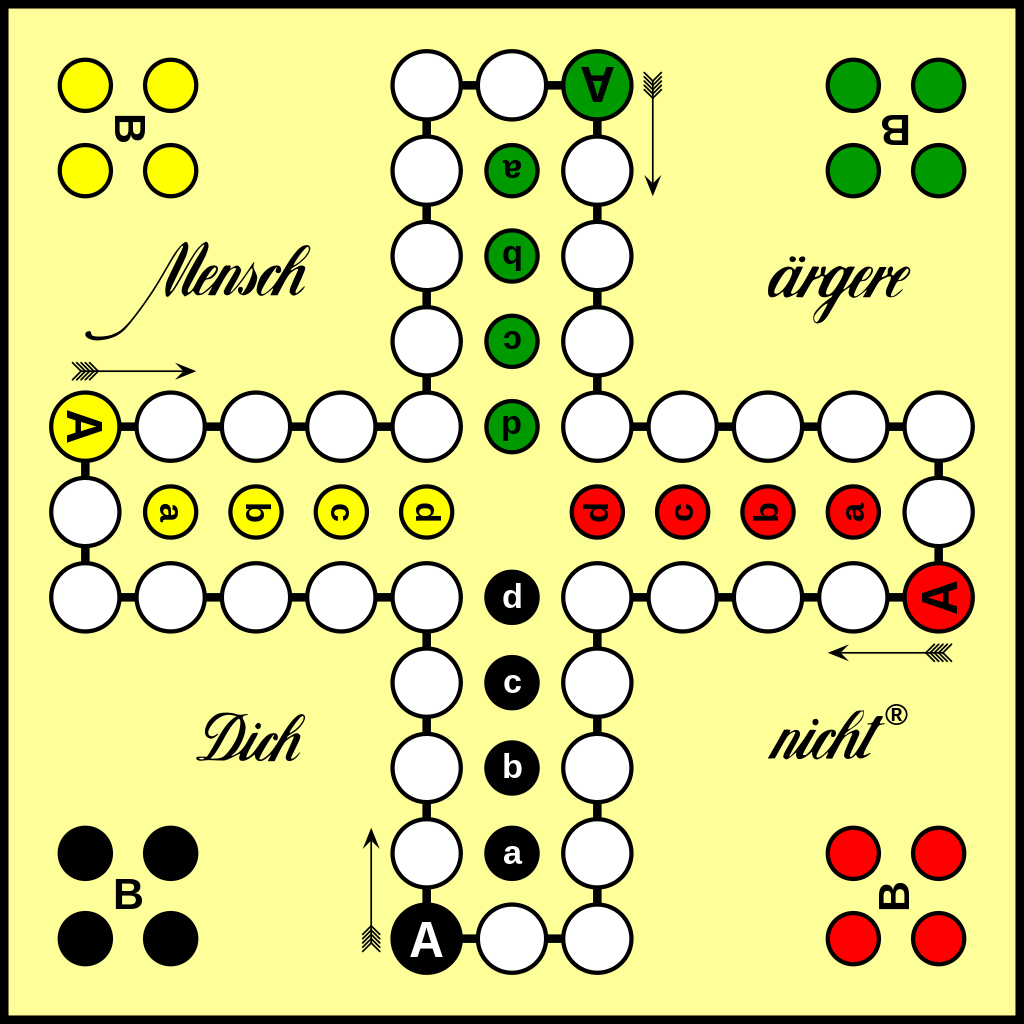
\includegraphics[width=0.7\textwidth]{images/Figure1}
    \caption{The board}
    \label{fig:board}
\end{figure}


The board is made up of 72 tiles - of which 48 are relevant to any single player.
The 4 color-coded fields of 4 tiles each, labeled with a capital B in each corner of the board, are the starting positions for
each player's 4 pieces. At the start of the game every piece is stuck here until a 6 is rolled, any other number will result in a null turn. These 4 tiles with be referred to as the "purgatory". Once a 6 is rolled however, the player is allowed to move one piece onto their color-coded starting tile, labeled with a capital A. From here an arrow indicates the starting direction. 
The 40, mostly white tiles, all connected by black lines, make up the main playing field.
Here a player needs to move towards making a full loop around the plus-shaped field as fast as possible.
Once a number is rolled that would put a piece onto or beyond the starting tile again, the piece instead starts moving into
the color-coded "abcd-tiles", which will be referred to as such from now on and represent the goal for each piece.
The letter a piece lands on is irrelevant. The game is finished when one player has filled out all of their abcd-tiles.

The aggravating mechanic that leads to the games iconic title comes from the interaction between different players. If a number is rolled that would make on piece move onto a tile that is occupied by a different
players piece, that piece will then be knocked out and forced to move back into the purgatory.
If a piece were to land on a tile occupied by another piece of the same team however, the turn is nullified instead.

These straight-forward but entertaining rules have ensured this games staying power over many generations, but for
our goal here we will discard its fundamental core - the player interaction - entirely.



\subsection{The problem}
Based on the rules of the game it is easy to assume that the quickest way to win would be to constantly roll a 6.
But what if we do not care about the "quickest" way and instead focus on the "shortest" way?
Every piece needs to be moved to it's new rolled position, but there is no rule requiring that movement to follow the path.
Instead, often, players will just move the piece in a straight line towards a tile and thereby skipping a large piece of the path. 

\begin{figure}[htbp]
    \centering
    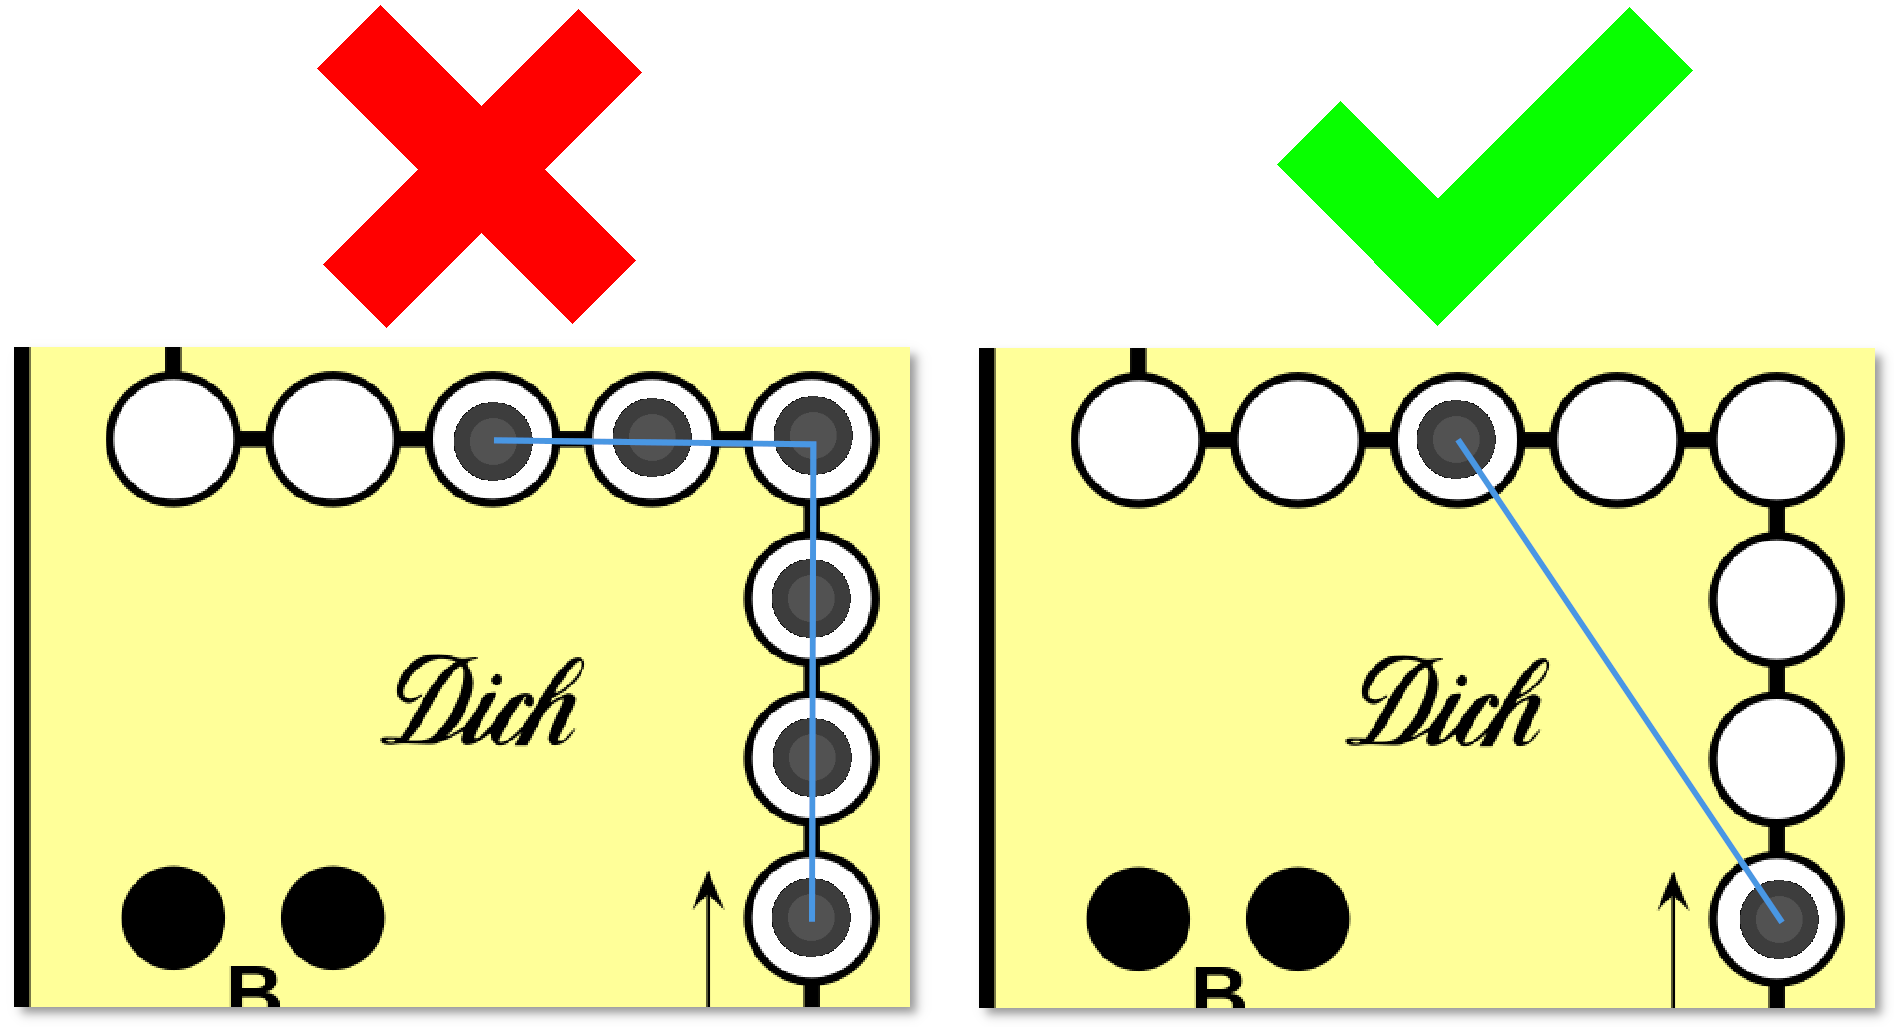
\includegraphics[width=0.6\textwidth]{images/Figure2}
    \caption{Shortcuts}
    \label{fig:shortcuts}
\end{figure}

One could wonder about the minimum amount of physical movement required to win a game if every roll is optimized towards skipping the maximum amount of tiles in a straight path. Since we only want to find the absolute best case scenario, we can completely ignore the other players. Ideally they never roll a 6 and stay in purgatory forever.


\section{Computability}\label{sec:computability}
The goal is to make a program that finds the shortest path fitting our description. Let us take a closer look into what kind of challenges this task will provide and what variables need to be accounted for.

Before even beginning to think about writing a program we need to assure ourselves that the problem is conceptually computable within a reasonable time frame.
The naive approach would be to simply loop through every possible outcome of the game and compare the length of all the paths
taken.
Every turn there are 6 different numbers that can be rolled. Additionally, for each of these 6 numbers there are 4 different outcomes depending on which piece the player chooses to move.
\[
    N_{Outcomes~per~turn} = 6_{Different~rolls} \cdot 4_{Pieces} = 24
\]
Of course, once some of the pieces are finished and can no longer move, N will change. This will be ignored for now however.

The number of turns to finish a game, when ignoring other players, can be assumed to be 4 times the amount needed for a single piece to finish. For simplicity's sake we can assume that average amount of turns for one piece will be the number of tiles divided by the average roll. When combining both of these terms we need to finish by rounding up to the next highest integer.
\[
    T_{Number~of~turns} =  \lceil \frac{44_{Tiles}}{3_{Average~Roll}} \cdot 4_{Pieces} \rceil
    =  59
\]

For each of the N outcomes per turn there will be N new outcomes, for which there will be N outcomes again and so forth until the game is finished after about T iterations. That means the amount of positions that need to be checked to find the shortest path via the naive approach would be N times N times N times N.... until all pieces are finished, in other words, N raised to T. Recall that we are ignoring the change in N resulting from less pieces being available to choose from over time.
\[
    P_{Positions} =  N^T = 24^{59} = 2.70684421 \cdot 10^{81}
\]

As you can see, this is a horrendously large number. In fact, it can be compared to the amount of particles in our universe, which is estimated to be around $10^{78}$ to $10^{82}$. Clearly, the naive approach will not work.

One way to improve upon this method would be decreasing N. Luckily, there is actually no reason to even consider which of the 4 pieces to move each turn, as the position of one piece can never be beneficial to another of the same team. This means we can safely only move on piece towards it's goal at a time and thereby get rid of the factor 4 in the equation for N.
\[
    N_{Outcomes~per~turn} = 6_{Different~rolls}
\]
\[
    P_{Positions} =  N^T = 6^{59} =8.145613\ \cdot 10^{45}
\]

This is a lot better but still way out of the range of easy computability.
However, N is not the only number that can be decreased by ignoring piece interaction. We can separate each of the 4 pieces' laps around the board into discrete problems to solve by having one piece on the main board at a time and the others either in purgatory or on the abcd-tiles.
\[
    S_{Purgatory} = 4_{Pieces} - F_{abcd}
\]
That means the problem boils down to finding the 4 shortest paths from the starting position to each of the 4 abcd-tiles.
Therefore we can remove the multiplication by the number of pieces from T and instead add it to the term for P.
\[
    T_{Turns~per~piece} =  \lceil \frac{44_{Tiles}}{3_{Average~Roll}}\rceil
    =  15
\]
\[
    P_{Number~of~positions} =  4_{Pieces} \cdot N^T = 4 \cdot 6^{15} = 1.88073994 \cdot 10^{12}
\]
P now seems computable. If we were able to write a program that can check 10 million positions in a second, it would take about
52 hours to complete. This will be optimized further of course, but for now we can be assured that the problem can actually be solved.


\section{Solving the problem}

\subsection{The idea}
The goal is to construct a program that is capable of not only finding the shortest path, but also doing so within a reasonable time-frame. Therefore it is best to begin by getting an overview over all the requirements such a program must fulfill and how they could conceptually be implemented. Let us begin by specifying a few constants to work with from now on. Since there is no constant agreed upon measurement for Mensch-ärgere-Dich-nicht boards, the program will be working with measurements generalized as "units".
\begin{itemize}
    \item The board size will be 10,000x10,000 units.
    \item The distance between two adjacent tiles on the main board will always be 850 units.
    \item The program will assume the role of player black, putting it's starting position A at (4170, 9170). Here (0,0) lies at the top left of the board.
\end{itemize}

Ideally the program should calculate all distances ahead of time so they can simply be looked up in a table while the shortest path is being searched. That may sound like a very large table at first, but any one tile only needs to calculate the distance to 6 neighbors as any distance to tiles further than 6 away will never be necessary when playing with a normal die. Therefore our list would not be longer than 40 tiles times 6 neighbors, or 240 entries. It is definitely more efficient to save 240 entries once and then looking them up instead of doing millions or billions of the same calculation over and over again while different positions are being searched through.

Additionally, the one set of distances that can be guaranteed to be included in the shortest path are those required to move each piece to the starting position. Since the tiles in the purgatory are (3,0), (4,0), (3,1), (4,1) tiles away from tile A and the tile distance is 850 units, the minimum total movement to the starting position when rounded up is:

\[
	\lceil 3\cdot850\ +\ 4\cdot850\ +\ \sqrt{\left(3\cdot850\right)^{2}+850^{2}}+\ \sqrt{\left(4\cdot850\right)^{2}+850^{2}}\rceil = 12143
\]

\newpage

Now we can begin specifying the conceptual program structure.
There should be a main loop that calls a function to find the shortest path for each of the 4 starting positions to their respective abcd-tile and then adds them up together.

\begin{figure}[htbp]
    \centering
    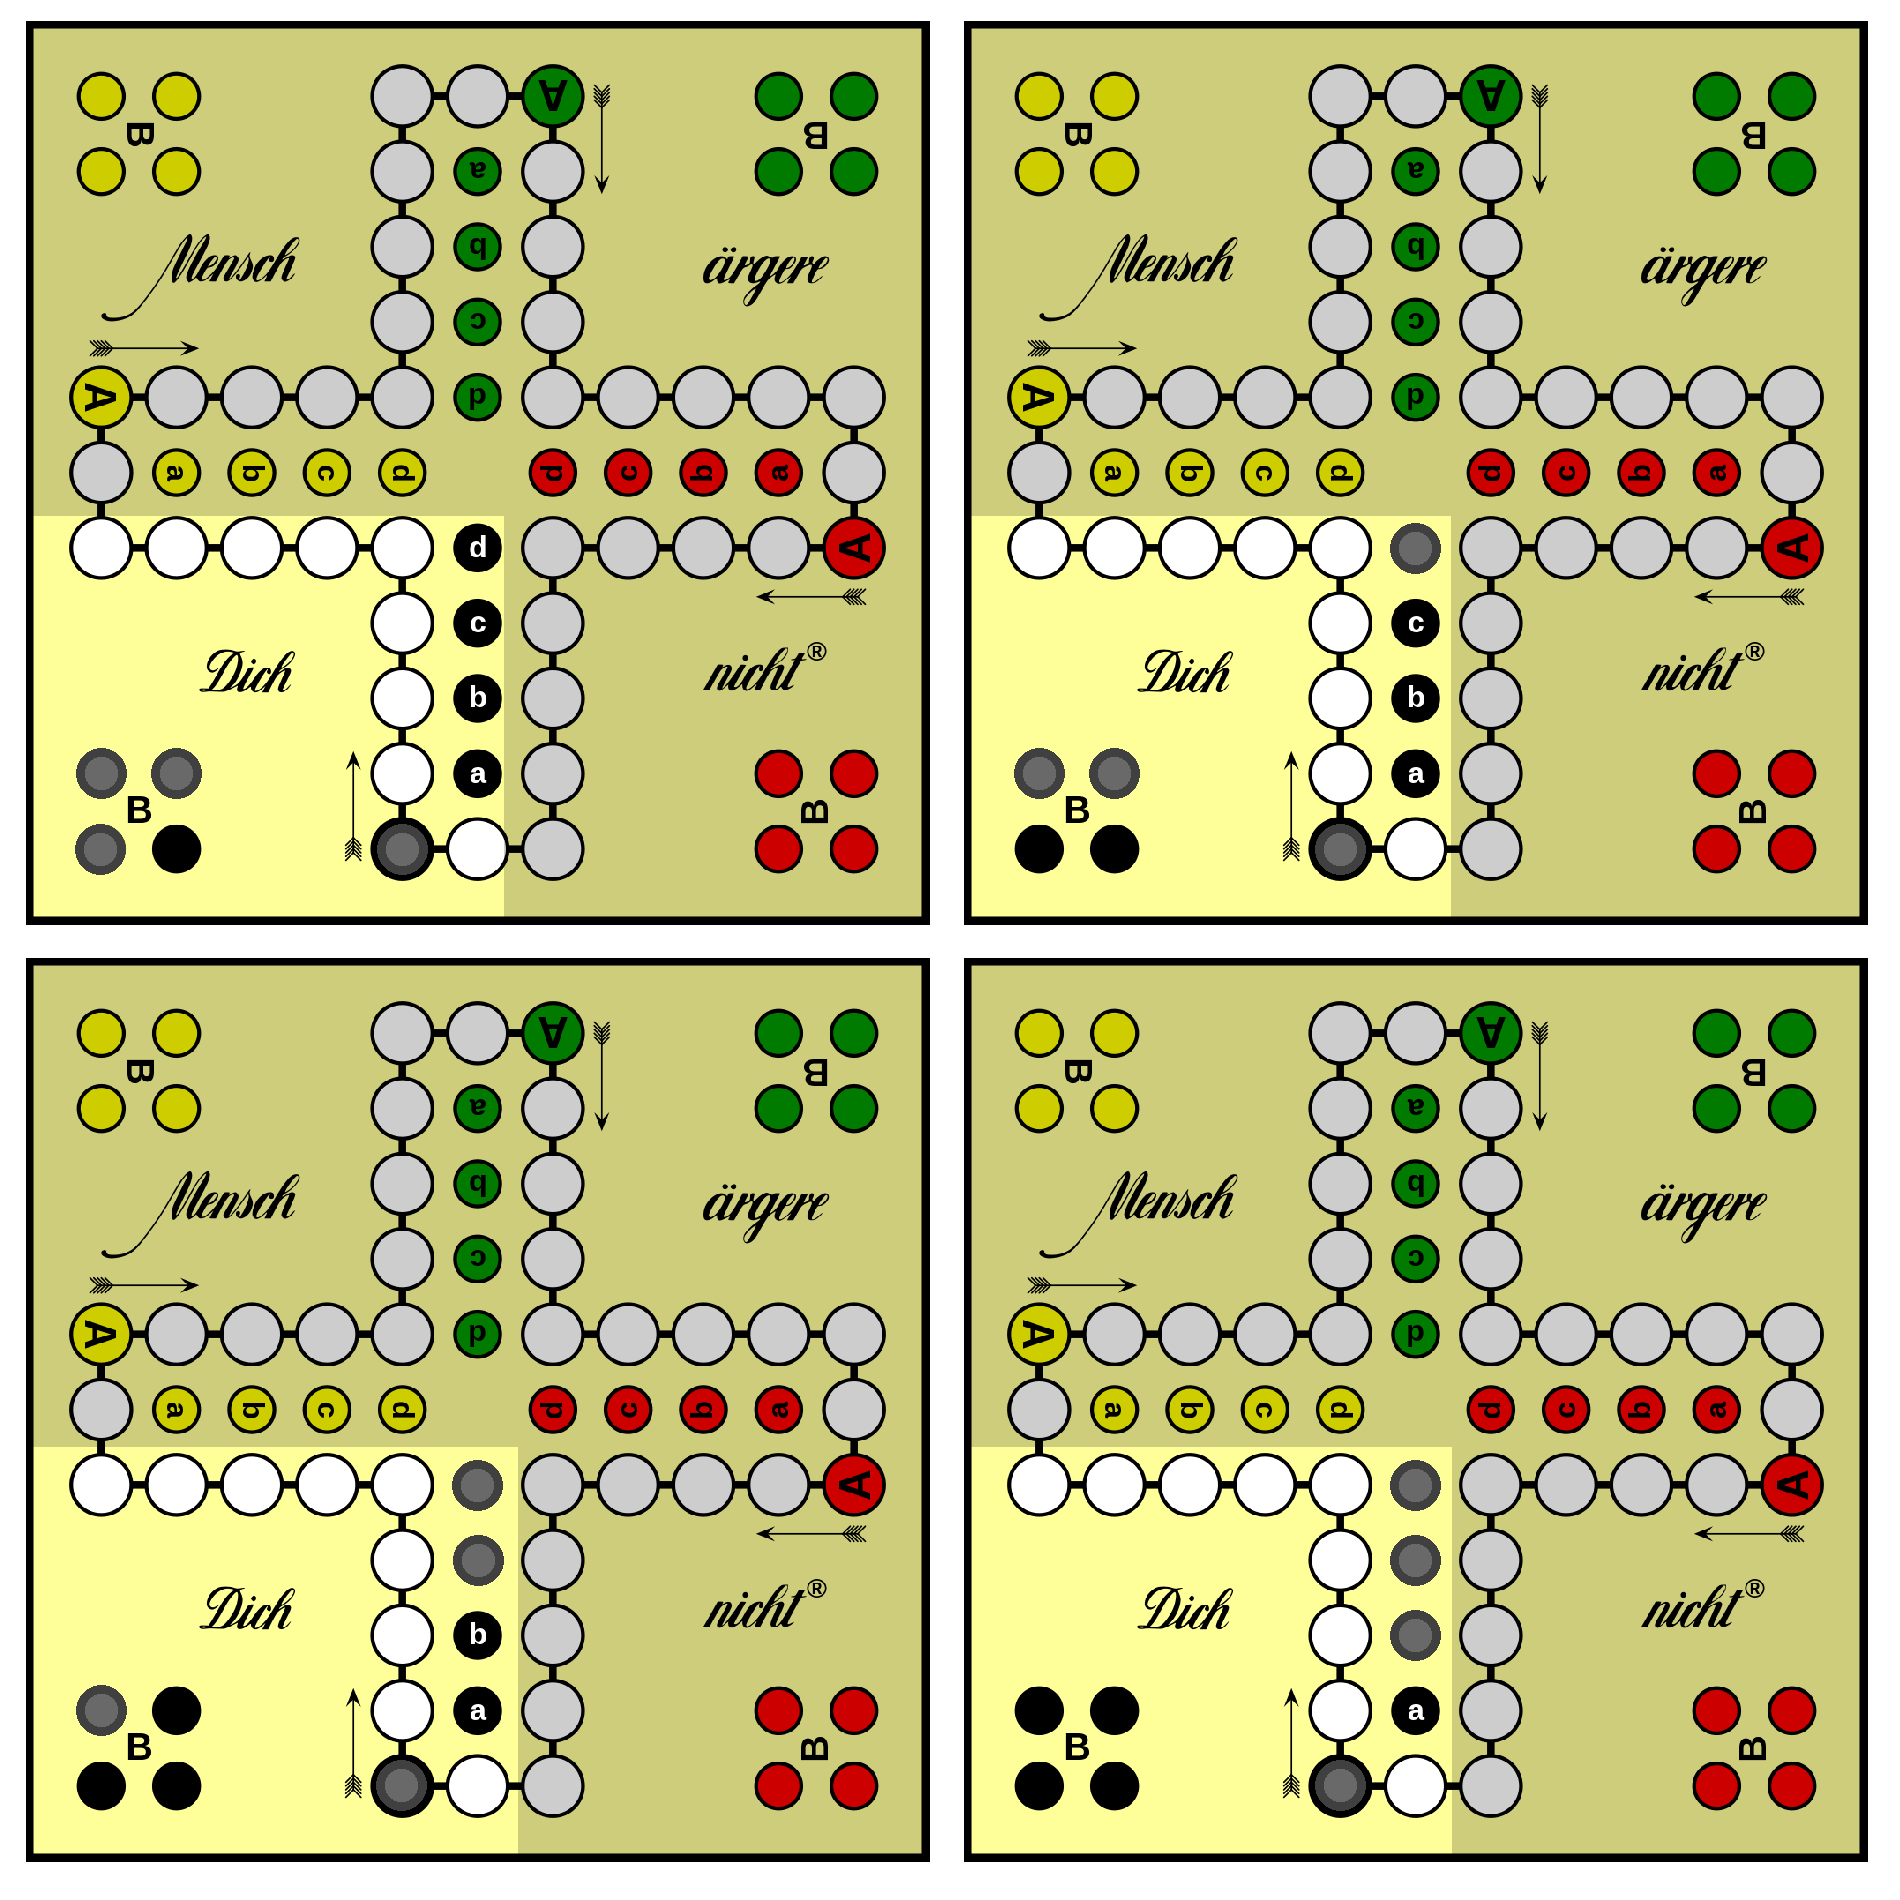
\includegraphics[width=0.6\textwidth]{images/Figure3}
    \caption{Starting positions}
    \label{fig:startpos}
\end{figure}

The reason for filling up the abcd-tiles starting from d at the very back is to prevent pieces from getting in the way of each other and thereby blocking the shortest path.

\begin{figure}[htbp]
    \centering
    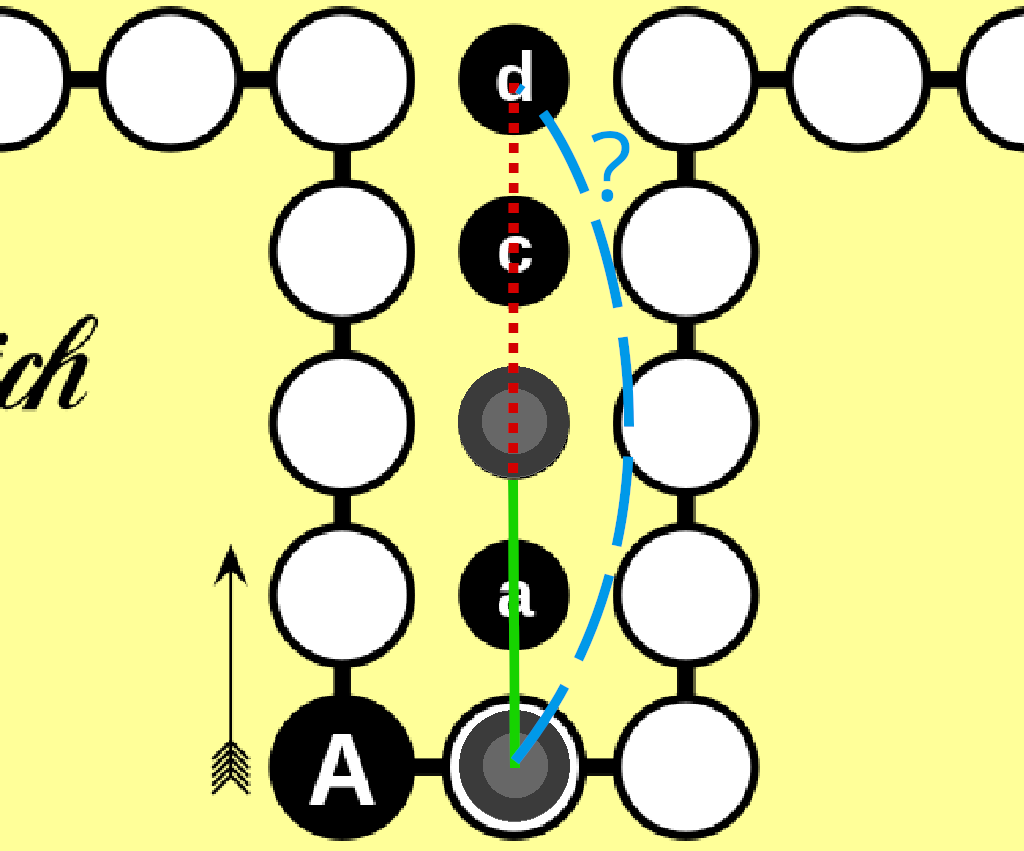
\includegraphics[width=0.3\textwidth]{images/Figure4}
    \caption{Blocked path}
    \label{fig:blockedpath}
\end{figure}

\newpage

The function finding the shortest path for a single starting position should operate recursively. It should take a specific position as well as the distance moved towards that position so far and then call itself six times and thereby looping over it's "sub-trees".
A sub-tree in this context is simply all the positions that follow a specific roll from a specific position when the total series of possible choices is imagined as a tree with it's roots at the starting position.

\begin{figure}[htbp]
    \centering
    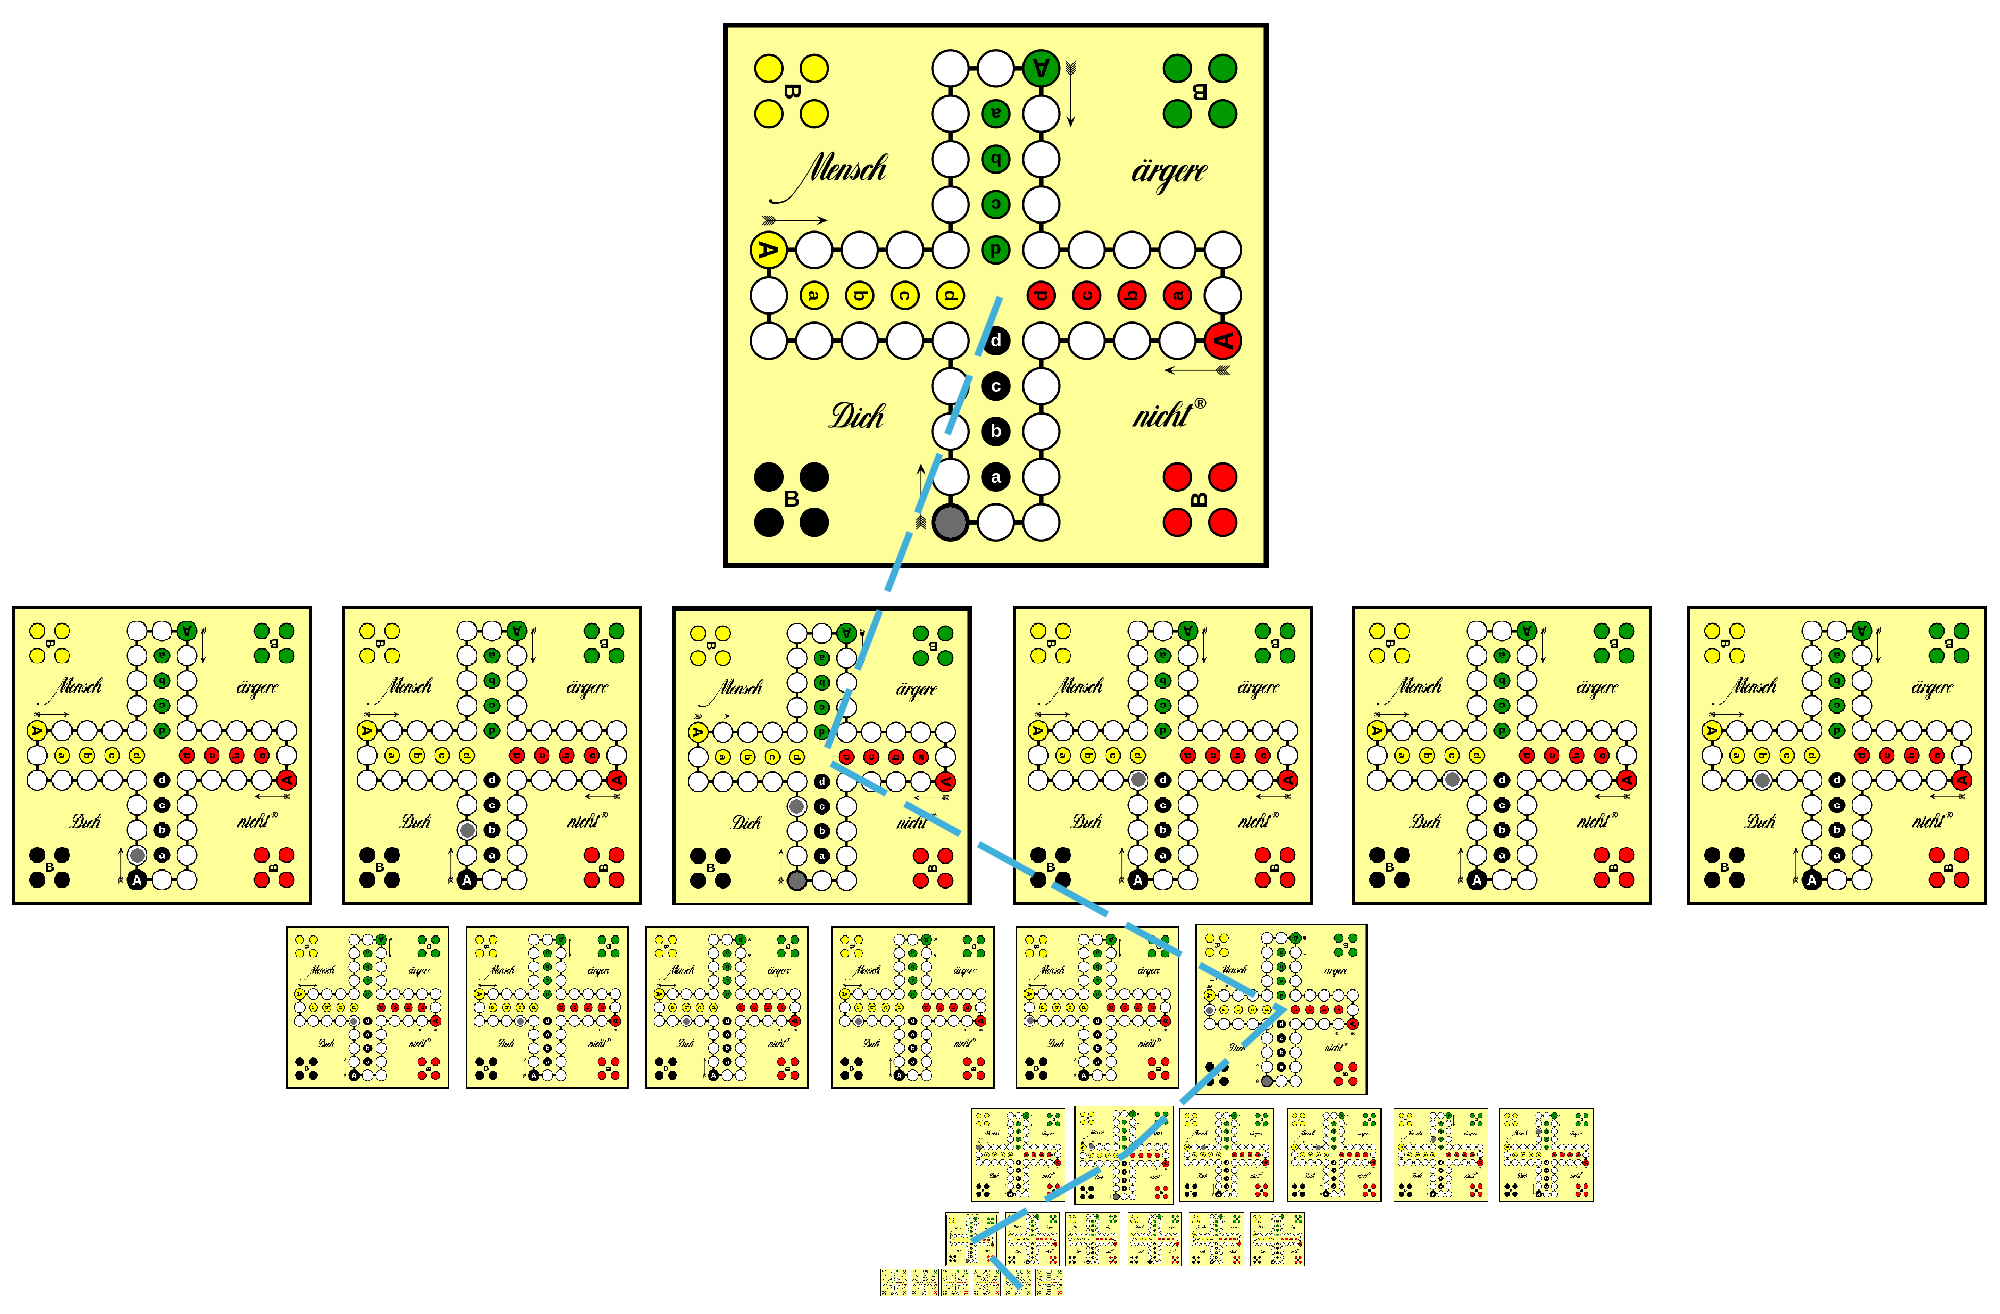
\includegraphics[width=1\textwidth]{images/Figure5}
    \caption{Singe path in tree}
    \label{fig:pathintree}
\end{figure}

The loop over the sub-trees of each position should start at 6 and count down. Rolling lower can only lead to shorter paths if it is not already possible to move to the goal in a straight line within one turn. Therefore, if a roll lands on the correct abcd tile it is guaranteed that it will be the shortest path to goal from the current position. In that case any lower rolls and their sub-trees can be ignored.

We should also stop going into further sub-trees if the current distance moved is already larger than that of the shortest path found so far. Although there is no way to tell how many positions that will exclude ahead of time, it is definitely an essential part of optimization and could save billions of unnecessary calculations depending on how early the final shortest path is found.

There will be more specifics that become apparent as soon as we start implementing these concepts in code of course, but for now this should be a solid guideline for how to construct the program. But one more thing needs to be considered first.

\subsection{The bit-board}
We want to save the current position and the distance moved for every function call in the position-tree, however, as seen in Section 2 - Computability, that could take up an incredibly large amount of space if we are not careful with what data structure we choose.
There needs to be a way to save both position and distance in a relatively compact and fast but also still easy to understand way.

Ideally the function should only receive a single, non-pointer variable. That variable should also be fast at being read from or written to. 
Computer are very fast at doing bit-wise operations, to the point where every other operation needs to be translated down into bit-wise operations. If both position and distance could be saved in a single number that could then be modified and read from using bit-wise operators, that structure would certainly satisfy our criteria.

A lot of the upcoming choices come down to personal preference. I have decided that I want a position to be represented by having each tile correspond to a bit. If the bit is a 0, it is empty. If it is a 1, there is a piece on the tile. Since there are 48 relevant tiles the use of a 32-bit number is out of the question. Since the next higher standardized type is a 64-bit number, we will have to stick with that, using the first 48 bits for the board state.

That leaves us with exactly 16 bits at the end. This space can be used for storing the amount of space moved up to the current position. Since we know every piece will receive it's own bit-board and thereby count only it's own movement, 16 bits are all we need. The distance between two tiles is 850 units while an unsigned 16 bit integer can represent numbers from 0 to 65536.
\[
    Maximum~worst~case~tile ~movements = \frac{65536_{uint16~limit}}{850_{Board~side~length}} = 77.10117
\]
This means we can store the worst case zero shortcut movement over a board with almost twice the amount of tiles of the original board for every single piece. Therefore, as long as we stick to keeping distance counting separated between the pieces, there is no need to worry about running out of space.

\subsection{The code}


\section{Discussion}

\subsection{Results}

\subsection{Runtime}
In the final version of the program the \text{handle\_piece()} function is called \newline 14 282 614 times in total, leading to an average runtime of 0.5 seconds on my AMD Ryzen 9 5950x CPU. This is quite remarkable when compared to the numbers calculated in Section 2 - Computability. However, exiting a branch once it has been calculated that there can no longer be a shorter path than the current shortest in this branch by using the  \text{min\_units\_per\_square} constant could be considered cheating. After all, there was no way for me to be fully confident in it's validity before running the program.
If we take out that optimization the program calls the function 660 449 985 times and runs for 22 seconds.


\end{document}